\documentclass[12pt,a4paper]{article}

\usepackage{fontspec}
\usepackage[polish]{babel}
\usepackage{amsmath}
\usepackage{array}
\usepackage{booktabs}
\usepackage{caption}
\usepackage{float}
\usepackage{geometry}
\usepackage{graphicx}
\usepackage{hyperref}
\usepackage{longtable}
\usepackage{xcolor}

\geometry{margin=2.5cm}
\defaultfontfeatures{Ligatures=TeX}
\setmainfont{Arial}
\hypersetup{
  colorlinks=true,
  linkcolor=black,
  urlcolor=blue,
  citecolor=black
}
\setlength{\parskip}{0.55em}
\setlength{\parindent}{0pt}
\renewcommand{\arraystretch}{1.18}
\sloppy

\title{Raport projektowy: klasyfikacja obrazów pomieszczeń z wykorzystaniem sieci neuronowych}
\author{Michał Dyło, Agnieszka Wardak}
\date{\today}

\begin{document}
\maketitle

\section{Wstęp i opis zagadnienia}

Celem projektu było zbudowanie i porównanie modeli głębokiego uczenia do klasyfikacji obrazów pomieszczeń. Rozważany problem należy do klasyfikacji wieloklasowej obrazów RGB: dla danego zdjęcia model ma wskazać typ pomieszczenia. W finalnej wersji eksperymentu rozpoznawano cztery klasy: \texttt{bed}, \texttt{din}, \texttt{kitchen} oraz \texttt{living}.

Zadanie jest trudniejsze niż klasyfikacja prostych obiektów, ponieważ klasy nie są definiowane przez pojedynczy charakterystyczny element. Sypialnia, salon i jadalnia mogą zawierać podobne meble, a granica między kuchnią i jadalnią bywa nieostra. Dodatkowo zdjęcia różnią się oświetleniem, perspektywą, stylem wnętrza, liczbą widocznych obiektów i stopniem uporządkowania sceny. Oznacza to, że model musi uczyć się zarówno lokalnych cech obrazu, jak i szerszego kontekstu przestrzennego.

Porównano trzy grupy modeli:
\begin{itemize}
  \item MLP jako prosty model bazowy pracujący na spłaszczonych pikselach,
  \item własną sieć konwolucyjną typu ResNet trenowaną od zera bez augmentacji,
  \item tę samą rodzinę sieci konwolucyjnych trenowaną z augmentacją danych oraz wariant ensemble.
\end{itemize}

Ważnym założeniem było to, że modele CNN nie korzystają z transfer learningu ani gotowych wag. Sieci były trenowane od zera, dzięki czemu porównanie między zwykłym CNN a CNN z augmentacją dotyczy faktycznie wpływu procedury uczenia i przetwarzania danych, a nie użycia wcześniej wytrenowanego modelu.

\section{Opis i eksploracyjna analiza danych}

Wykorzystano zbiór \textit{House Rooms \& Streets Image Dataset} z Kaggle \cite{kaggle_dataset}. Dataset zawiera katalogi \texttt{house\_data} oraz \texttt{street\_data}; w projekcie użyto wyłącznie katalogu \texttt{house\_data}, ponieważ dotyczył zdjęć wnętrz.

W katalogu \texttt{house\_data} znajdowało się 5249 obrazów w pięciu klasach. Etykieta była zapisana w nazwie pliku jako prefiks, np. \texttt{bed\_...jpg}. Liczebności klas przedstawiono w tabeli \ref{tab:class_counts_all}.

\begin{table}[H]
\centering
\caption{Liczebność klas w pełnym katalogu \texttt{house\_data}.}
\label{tab:class_counts_all}
\begin{tabular}{lr}
\toprule
Klasa & Liczba obrazów \\
\midrule
\texttt{bath} & 605 \\
\texttt{bed} & 1248 \\
\texttt{din} & 1158 \\
\texttt{kitchen} & 965 \\
\texttt{living} & 1273 \\
\midrule
Razem & 5249 \\
\bottomrule
\end{tabular}
\end{table}

Klasę \texttt{bath} usunięto z finalnego eksperymentu, aby zachować zgodność z wcześniejszą wersją notebooka oraz skupić się na klasach o większej wzajemnej niejednoznaczności wizualnej. Po usunięciu tej klasy pozostały 4644 obrazy. Dane podzielono stratyfikacyjnie na zbiory treningowy, walidacyjny i testowy w proporcji 70\%/15\%/15\%. Ten sam podział był używany dla wszystkich modeli, co umożliwia bezpośrednie porównanie wyników.

\begin{table}[H]
\centering
\caption{Stratyfikowany podział danych po usunięciu klasy \texttt{bath}.}
\label{tab:split_counts}
\begin{tabular}{lrrrrr}
\toprule
Podzbiór & \texttt{bed} & \texttt{din} & \texttt{kitchen} & \texttt{living} & Razem \\
\midrule
Treningowy & 873 & 811 & 675 & 891 & 3250 \\
Walidacyjny & 187 & 174 & 145 & 191 & 697 \\
Testowy & 188 & 173 & 145 & 191 & 697 \\
\bottomrule
\end{tabular}
\end{table}

\begin{figure}[H]
\centering
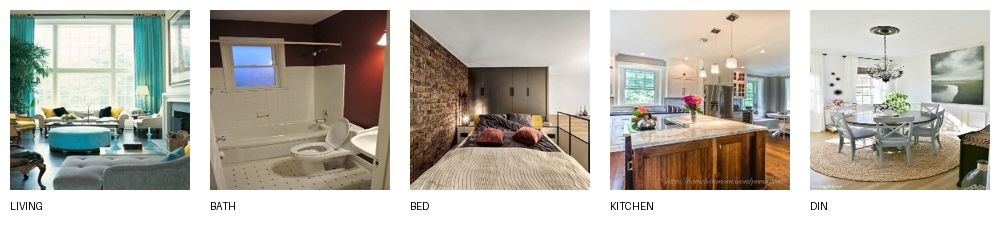
\includegraphics[width=0.95\textwidth]{figures/sample_rooms_grid.png}
\caption{Przykładowe obrazy z czterech klas użytych w eksperymencie.}
\label{fig:samples}
\end{figure}

Podczas eksploracji danych zauważono, że klasy są dość zbalansowane, ale nie idealnie. Najmniej przykładów ma klasa \texttt{kitchen}, a najwięcej \texttt{living}. Różnice nie są na tyle duże, aby wymagały agresywnego oversamplingu, natomiast w funkcji straty zastosowano wagi klas obliczone na podstawie liczebności zbioru treningowego. Dzięki temu błędy w mniej licznej klasie nie są marginalizowane.

Preprocessing był zależny od modelu:
\begin{itemize}
  \item MLP używał obrazów \(96 \times 96\), ponieważ większe wejście znacznie zwiększa liczbę wag w pierwszej warstwie gęstej.
  \item Zwykły CNN bez augmentacji był oceniany dla najlepszego wariantu \(224 \times 224\).
  \item Najlepsze modele CNN z augmentacją używały obrazów \(256 \times 256\).
\end{itemize}

Dla wszystkich modeli obrazy konwertowano do RGB, skalowano do odpowiedniego rozmiaru i normalizowano przy użyciu średniej oraz odchylenia standardowego ImageNet:
\[
\mu=(0.485, 0.456, 0.406), \qquad \sigma=(0.229, 0.224, 0.225).
\]
Normalizacja nie oznacza użycia transfer learningu; jest jedynie standardowym przeskalowaniem kanałów wejściowych.

\section{Architektury sieci i procedura uczenia}

\subsection{Funkcja straty i metryki}

Modele trenowano w PyTorch. Minimalizowaną funkcją straty była ważona entropia krzyżowa z label smoothing:
\[
\mathcal{L}(x, y) = - \sum_{c=1}^{C} w_c \tilde{y}_c \log p_c,
\]
gdzie \(w_c\) jest wagą klasy, \(p_c\) prawdopodobieństwem przewidywanym przez model, a \(\tilde{y}\) wygładzoną etykietą. W modelach z MixUp/CutMix funkcja straty obsługiwała również miękkie etykiety.

Jako główne metryki raportowano accuracy oraz macro F1. Macro F1 jest szczególnie istotne, ponieważ liczy średnią jakość po klasach, a nie po przykładach, więc lepiej pokazuje, czy model działa równomiernie na wszystkich kategoriach.

\subsection{Model bazowy MLP}

MLP użyto jako punktu odniesienia. Model nie wykorzystuje lokalnej struktury obrazu, ponieważ po warstwie \texttt{Flatten} traktuje obraz jako jeden długi wektor pikseli. Architektura MLP była następująca:

\begin{table}[H]
\centering
\caption{Architektura modelu MLP.}
\label{tab:mlp_arch}
\begin{tabular}{ll}
\toprule
Element & Opis \\
\midrule
Wejście & obraz RGB \(96 \times 96\), czyli 27648 cech po spłaszczeniu \\
Warstwa 1 & Linear(27648, 1024) + BatchNorm + ReLU + Dropout(0.50) \\
Warstwa 2 & Linear(1024, 512) + BatchNorm + ReLU + Dropout(0.50) \\
Warstwa 3 & Linear(512, 256) + BatchNorm + ReLU + Dropout(0.375) \\
Wyjście & Linear(256, 4) \\
\bottomrule
\end{tabular}
\end{table}

Najlepszy wariant MLP uzyskano dla rozmiaru obrazu \(96 \times 96\), learning rate \(5 \cdot 10^{-4}\), weight decay \(10^{-4}\), dropout 0.50 i label smoothing 0.03. Model był trenowany z early stopping; najlepszy punkt walidacyjny wystąpił w 28. epoce.

\subsection{Własna sieć CNN typu ResNet}

Główny model konwolucyjny to własna architektura \texttt{RoomResNet}, trenowana od zera. Nie użyto gotowej sieci ani wag pretrenowanych. Architektura łączy bloki rezydualne, BatchNorm, aktywację SiLU, Squeeze-and-Excitation oraz global average pooling.

Pojedynczy blok rezydualny ma postać:
\[
\begin{aligned}
x &\rightarrow \text{Conv}_{3\times3} \rightarrow \text{BN} \rightarrow \text{SiLU}
\rightarrow \text{Dropout2D} \\
  &\rightarrow \text{Conv}_{3\times3} \rightarrow \text{BN}
\rightarrow \text{SE}
\rightarrow +\text{shortcut}
\rightarrow \text{SiLU}.
\end{aligned}
\]
Jeżeli liczba kanałów lub rozdzielczość zmienia się między wejściem i wyjściem bloku, shortcut zawiera konwolucję \(1 \times 1\) ze stride.

Moduł Squeeze-and-Excitation \cite{senet} najpierw wykonuje global average pooling, następnie przechodzi przez dwie konwolucje \(1 \times 1\) i funkcję sigmoid. W ten sposób model uczy się ważenia kanałów cech.

\begin{table}[H]
\centering
\caption{Konfiguracje architektury \texttt{RoomResNet}.}
\label{tab:roomresnet_configs}
\begin{tabular}{lrrrr}
\toprule
Wariant & Kanały stem & Kanały etapów & Liczba bloków & Parametry \\
\midrule
small & 32 & 48, 96, 192, 320 & 2, 2, 2, 2 & ok. 5.08 mln \\
medium & 48 & 64, 128, 256, 384 & 2, 2, 3, 2 & ok. 9.15 mln \\
large & 64 & 80, 160, 320, 512 & 2, 3, 4, 2 & ok. 17.63 mln \\
\bottomrule
\end{tabular}
\end{table}

Finalnie najlepsze wyniki dawał wariant \texttt{large}. Jego dokładna struktura składa się z:
\begin{itemize}
  \item dwóch konwolucji wejściowych \(3 \times 3\) z 64 kanałami,
  \item czterech etapów rezydualnych o kanałach 80, 160, 320 i 512,
  \item liczby bloków w etapach równej odpowiednio 2, 3, 4 i 2,
  \item global average pooling do wektora 512,
  \item klasyfikatora Linear(512, 256) + SiLU + Dropout + Linear(256, 4).
\end{itemize}

Wariant CNN bez augmentacji był trenowany bez jakichkolwiek losowych modyfikacji obrazu. To ważne rozróżnienie: zwykły CNN miał służyć jako kontrola, a CNN+aug jako wariant pokazujący wpływ augmentacji i regularizacji danych.

\subsection{CNN z augmentacją danych}

Wariant CNN+aug używa tej samej rodziny architektur \texttt{RoomResNet}. Różni się procedurą treningową i przetwarzaniem danych. W profilu augmentacji \texttt{strong} zastosowano:
\begin{itemize}
  \item RandomResizedCrop do rozmiaru wejściowego, skala 0.62--1.00, proporcje 0.80--1.25,
  \item losowe odbicie poziome,
  \item ColorJitter dla jasności, kontrastu, nasycenia i barwy,
  \item RandAugment z dwoma operacjami o sile 7,
  \item losową skalę szarości, autokontrast i zmianę ostrości,
  \item GaussianBlur,
  \item RandomAffine oraz RandomPerspective,
  \item RandomErasing po normalizacji.
\end{itemize}

Dodatkowo dla najlepszych modeli użyto MixUp \cite{mixup} i CutMix \cite{cutmix}. MixUp tworzy wypukłą kombinację dwóch obrazów i ich etykiet, a CutMix wkleja fragment jednego obrazu do drugiego i miesza etykiety proporcjonalnie do pola wklejonego fragmentu. Najlepszy model CNN+aug używał:
\[
\alpha_{\text{mixup}}=0.2, \qquad \alpha_{\text{cutmix}}=1.0, \qquad p_{\text{mix}}=0.45.
\]

W ocenie modeli CNN+aug zastosowano test-time augmentation (TTA). Dla każdego obrazu wykonano 5 predykcji: jedną deterministyczną oraz dodatkowe losowe cropy/odbicia, a następnie uśredniono prawdopodobieństwa. Zwykły CNN i MLP były oceniane bez TTA.

\subsection{Procedura uczenia i strojenie hiperparametrów}

Wszystkie modele trenowano z optymalizatorem AdamW \cite{adamw}. Maksymalną liczbę epok ustawiono wysoko, ale trening kończono przez early stopping na podstawie macro F1 na zbiorze walidacyjnym. Dzięki temu modele mogły trenować długo, ale nie wybierano wag z końca uczenia, jeśli walidacja przestawała się poprawiać.

Strojenie hiperparametrów wykonano etapowo:
\begin{itemize}
  \item dla MLP porównano warianty rozmiaru wejścia, learning rate, weight decay i dropout;
  \item dla zwykłego CNN przeszukano warianty \texttt{medium}/\texttt{large}, learning rate \(3 \cdot 10^{-4}\) i \(5 \cdot 10^{-4}\), weight decay \(5 \cdot 10^{-4}\) i \(10^{-3}\), dropout 0.40 i 0.50;
  \item dla CNN+aug wykonano grid search po learning rate, weight decay, dropout i prawdopodobieństwie MixUp/CutMix.
\end{itemize}

\begin{table}[H]
\centering
\caption{Najważniejsze hiperparametry najlepszego pojedynczego modelu CNN+aug.}
\label{tab:best_hparams}
\begin{tabular}{ll}
\toprule
Parametr & Wartość \\
\midrule
Architektura & \texttt{RoomResNet large} \\
Rozmiar wejścia & \(256 \times 256\) \\
Liczba parametrów & 17.63 mln \\
Learning rate & \(2 \cdot 10^{-4}\) \\
Weight decay & \(5 \cdot 10^{-4}\) \\
Dropout w głowie & 0.40 \\
Label smoothing & 0.10 \\
Scheduler & cosine decay z 12 epokami warmup \\
EMA wag & 0.999 \\
MixUp/CutMix & \(\alpha_{\text{mixup}}=0.2\), \(\alpha_{\text{cutmix}}=1.0\), \(p=0.45\) \\
TTA w ewaluacji & 5 predykcji na obraz \\
\bottomrule
\end{tabular}
\end{table}

Najlepszy pojedynczy model CNN+aug osiągnął najlepszy punkt walidacyjny w 206. epoce. W tym punkcie walidacyjne macro F1 wyniosło 0.8681, a accuracy 0.8694. Model trenowano łącznie 281 epok, po czym early stopping zatrzymał uczenie.

Oprócz pojedynczych modeli zbudowano ensemble trzech najlepszych modeli CNN+aug z grid searcha. Ensemble nie wymaga dodatkowego treningu: dla każdego obrazu liczone są prawdopodobieństwa trzech modeli, następnie są one uśredniane, a przewidywana klasa to argmax średniego wektora prawdopodobieństw. W ensemble użyto modeli:
\begin{itemize}
  \item \texttt{lr2e4\_wd5e4\_d40\_m45},
  \item \texttt{lr3e4\_wd5e4\_d40\_m30},
  \item \texttt{lr2e4\_wd5e4\_d45\_m45}.
\end{itemize}

\section{Wyniki}

Wyniki w tabeli \ref{tab:main_results} pochodzą z wykonanego notebooka ewaluacyjnego \texttt{evaluate\_trained\_models.ipynb}. Test obejmował 697 obrazów.

\begin{table}[H]
\centering
\caption{Porównanie wyników na zbiorze testowym.}
\label{tab:main_results}
\begin{tabular}{lrrr}
\toprule
Model & Accuracy & Macro F1 & TTA \\
\midrule
MLP & 40.89\% & 40.80\% & 1 \\
CNN bez augmentacji & 64.99\% & 65.23\% & 1 \\
Najlepszy pojedynczy CNN+aug & 88.81\% & 88.70\% & 5 \\
Ensemble top 3 CNN+aug & \textbf{89.81\%} & \textbf{89.70\%} & 5 \\
\bottomrule
\end{tabular}
\end{table}

Wyniki pokazują bardzo wyraźną różnicę między MLP a modelami konwolucyjnymi. MLP osiąga tylko 40.80\% macro F1, ponieważ po spłaszczeniu obrazu traci informację o lokalnym sąsiedztwie pikseli. Zwykły CNN poprawia wynik do 65.23\% macro F1, ale bardzo silnie przeucza się do zbioru treningowego. W jego historii treningowej accuracy treningowe dochodziło do prawie 100\%, podczas gdy walidacja pozostawała w okolicach 65\%.

Największy wzrost jakości daje augmentacja. Najlepszy pojedynczy model CNN+aug osiąga 88.70\% macro F1, czyli ponad 23 punkty procentowe więcej niż zwykły CNN. Ensemble trzech modeli poprawia wynik do 89.70\% macro F1.

\subsection{Wyniki per klasa}

\begin{table}[H]
\centering
\caption{Metryki per klasa dla finalnego ensemble.}
\label{tab:per_class_ensemble}
\begin{tabular}{lrrrr}
\toprule
Klasa & Precision & Recall & F1 & Support \\
\midrule
\texttt{bed} & 0.914 & 0.957 & 0.935 & 188 \\
\texttt{din} & 0.893 & 0.873 & 0.883 & 173 \\
\texttt{kitchen} & 0.868 & 0.910 & 0.889 & 145 \\
\texttt{living} & 0.911 & 0.853 & 0.881 & 191 \\
\bottomrule
\end{tabular}
\end{table}

Najłatwiejszą klasą dla finalnego modelu jest \texttt{bed}, dla której recall wynosi 95.7\%. Najtrudniejsze pozostają \texttt{din} oraz \texttt{living}; są to klasy często współwystępujące wizualnie, np. w otwartych przestrzeniach typu salon z jadalnią.

\subsection{Macierze pomyłek}

\begin{table}[H]
\centering
\caption{Macierz pomyłek finalnego ensemble. Wiersze oznaczają klasy prawdziwe, kolumny predykcje.}
\label{tab:cm_ensemble}
\begin{tabular}{lrrrr}
\toprule
 & \texttt{bed} & \texttt{din} & \texttt{kitchen} & \texttt{living} \\
\midrule
\texttt{bed} & 180 & 0 & 2 & 6 \\
\texttt{din} & 3 & 151 & 12 & 7 \\
\texttt{kitchen} & 2 & 8 & 132 & 3 \\
\texttt{living} & 12 & 10 & 6 & 163 \\
\bottomrule
\end{tabular}
\end{table}

\begin{figure}[H]
\centering
\includegraphics[width=0.70\textwidth]{python_training/outputs/reports/notebook_final_eval/ensemble_top3_cnn_aug_tta5/ensemble_top3_cnn_aug_tta5.test.confusion_matrix.png}
\caption{Macierz pomyłek finalnego ensemble zapisana przez notebook ewaluacyjny.}
\label{fig:cm_ensemble}
\end{figure}

Dla porównania, zwykły CNN bez augmentacji osiągał dużo niższy wynik i częściej mylił \texttt{living} z \texttt{bed} oraz \texttt{din}. Jego macierz pomyłek przedstawiono w tabeli \ref{tab:cm_cnn_plain}.

\begin{table}[H]
\centering
\caption{Macierz pomyłek najlepszego zwykłego CNN bez augmentacji.}
\label{tab:cm_cnn_plain}
\begin{tabular}{lrrrr}
\toprule
 & \texttt{bed} & \texttt{din} & \texttt{kitchen} & \texttt{living} \\
\midrule
\texttt{bed} & 135 & 9 & 10 & 34 \\
\texttt{din} & 14 & 107 & 17 & 35 \\
\texttt{kitchen} & 14 & 19 & 98 & 14 \\
\texttt{living} & 36 & 29 & 13 & 113 \\
\bottomrule
\end{tabular}
\end{table}

\section{Podsumowanie}

Projekt pokazuje, że dla klasyfikacji obrazów pomieszczeń sama architektura CNN nie wystarcza. Zwykły model konwolucyjny trenowany bez augmentacji uczy się zbioru treningowego bardzo dobrze, ale generalizuje ograniczenie. Wynik 65.23\% macro F1 wskazuje na silne przeuczenie.

Największą poprawę uzyskano przez połączenie kilku elementów: mocniejszej architektury rezydualnej, dużej rozdzielczości wejścia, silnej augmentacji, MixUp/CutMix, EMA wag, schedulera cosine z warmupem oraz TTA w ewaluacji. Najlepszy pojedynczy model CNN+aug osiągnął 88.70\% macro F1, a ensemble trzech modeli poprawił wynik do 89.70\% macro F1.

Najważniejsze wnioski:
\begin{itemize}
  \item MLP jest zbyt słaby dla tego zadania, ponieważ ignoruje przestrzenną strukturę obrazu.
  \item CNN bez augmentacji wyraźnie przewyższa MLP, ale nadal przeucza się do danych treningowych.
  \item Augmentacja jest kluczowym składnikiem rozwiązania; odpowiada za największy wzrost jakości.
  \item Ensemble daje dodatkową, mniejszą, ale stabilną poprawę względem najlepszego pojedynczego modelu.
  \item Najtrudniejsze pomyłki dotyczą klas semantycznie podobnych, zwłaszcza \texttt{din}, \texttt{kitchen} i \texttt{living}.
\end{itemize}

Dalszą poprawę można byłoby uzyskać przez ręczne przejrzenie błędnie sklasyfikowanych obrazów, dodatkową kalibrację ensemble oraz ewentualne wykorzystanie większej liczby seedów. W projekcie świadomie nie zastosowano transfer learningu; jego użycie prawdopodobnie mogłoby podnieść wynik, ale zmieniłoby charakter porównania.

\begin{thebibliography}{9}

\bibitem{kaggle_dataset}
Mikhail Ma, \textit{House Rooms \& Streets Image Dataset}, Kaggle.
\url{https://www.kaggle.com/datasets/mikhailma/house-rooms-streets-image-dataset}

\bibitem{pytorch}
Paszke, A. et al., \textit{PyTorch: An Imperative Style, High-Performance Deep Learning Library}, NeurIPS, 2019.

\bibitem{resnet}
He, K., Zhang, X., Ren, S., Sun, J., \textit{Deep Residual Learning for Image Recognition}, CVPR, 2016.

\bibitem{senet}
Hu, J., Shen, L., Sun, G., \textit{Squeeze-and-Excitation Networks}, CVPR, 2018.

\bibitem{adamw}
Loshchilov, I., Hutter, F., \textit{Decoupled Weight Decay Regularization}, ICLR, 2019.

\bibitem{mixup}
Zhang, H. et al., \textit{mixup: Beyond Empirical Risk Minimization}, ICLR, 2018.

\bibitem{cutmix}
Yun, S. et al., \textit{CutMix: Regularization Strategy to Train Strong Classifiers with Localizable Features}, ICCV, 2019.

\bibitem{randaugment}
Cubuk, E. D. et al., \textit{RandAugment: Practical Automated Data Augmentation with a Reduced Search Space}, CVPR Workshops, 2020.

\end{thebibliography}

\end{document}
